\documentclass{article}
\usepackage[margin=0.5in]{geometry}
\usepackage[utf8]{inputenc}
\usepackage{makecell}
\usepackage{caption}
\usepackage{svg}
\usepackage{relsize}
\usepackage{gensymb}

%\title{Ćwiczenie nr 0: Wahadło matematyczne}
%\author{Tomasz Buczek, Maciej Mucha }
%\date{Październik 2016}

\usepackage{natbib}
\usepackage{float}
\usepackage{graphicx}
\usepackage{graphics}
\usepackage{wrapfig}
\usepackage[polish]{babel}
\usepackage[T1]{fontenc}
\renewcommand{\arraystretch}{1.5}%
\captionsetup{justification=centering}

\begin{document}

%\maketitle
\begin{center}
   \setlength{\extrarowheight}{5pt}
    \begin{tabular}{|l|l|r|r|r|}
      \hline
      \textbf{Wydział} & \textbf{Imię i nazwisko:} & \textbf{Rok} & \textbf{Grupa} & \textbf{Zespół}\\ [10pt] \hline
      \makecell{Elektrotechniki, Automatyki,\\ Informatyki i Inżynierii Biomedycznej} & \makecell{1. Tomasz Buczek \\ 2. Maciej Mucha} & I & IV & IV \\ [10pt] \hline
      \makecell{\textbf{PRACOWNIA} \\ \textbf{FIZYCZNA} \\ \textbf{WFIiS AGH}} & \multicolumn{2}{c}{\textbf{\textsc{Wahadło fizyczne}}} &  & Ćwiczenie nr: 1 \\ [10pt]
      \hline
      Data wykoniania: & Data oddania: & Zwrot do popr. & Data oddania & Data zaliczenia \\ [25pt] \hline
      \multicolumn{5}{r}{OCENA: \hspace {2cm} }
    \end{tabular}
\end{center}

\section{Cel ćwiczenia}
Wyznaczenie modułu Younga dla różnych materiałów na podstawie pomiaru prędkości rozchodzenia się fali.

\section{Część teoretyczna}

\begin{wrapfigure}{r}{0.5\textwidth} 
     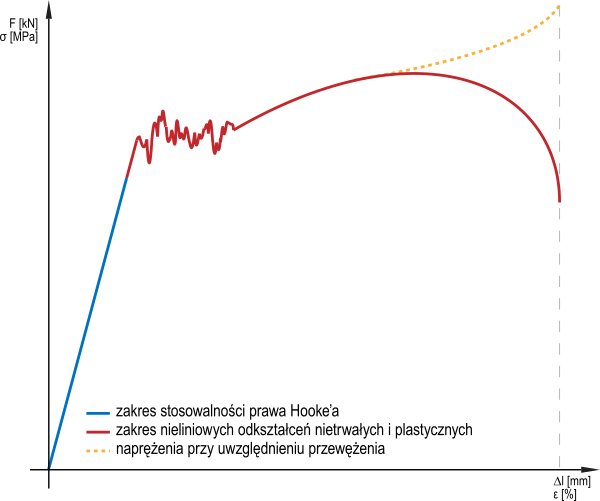
\includegraphics[scale=0.5]{wykres.jpg}
     \label{fig:my_label}
 \end{wrapfigure}
 
 Fala podłużna  to fala, w której drgania odbywają się w kierunku zgodnym z kierunkiem jej rozchodzenia się. 
 Opisuje ją równanie $$ y= Acos(\omega t \pm kx) $$
 
 Prawa Hooke'a: Odkształcenie jest wprost proporcjonalne do wywołującej je siły.
 \newline
 
 Opisuje to wzór: $$ \Delta l = \frac{Fl}{ES} $$
 $\Delta l$ - zmiana długości pręta, F - siła odkształcająca, l - długość, S - pole przekroju. \newline
 Współczynnik E to właśnie stała nazwana modułem Younga.
 
 Wyprowadzenie wzoru na moduł Younga, który będzie przydatny do późniejszych obliczeń.
 \newline
 Wychodząc od ogólnego wzoru na prawo Hooke'a: 
 $$ \sigma = \varepsilon E $$  $\sigma $ - naprężenie, $\varepsilon $ - odkształcenie względne
 $$ \varepsilon = \frac{\delta \Psi}{\delta x} $$
 \newline
Otrzymujemy wzór na  prędkość rozchodzenia się fali w pręcie: 
$$ v = \sqrt{\frac{E}{\rho}} $$
czyli $$ E = v^2\rho $$
\newline
W pręcie powstaje fala stojąca, odległość między węzłami fali stojące wynosi $ l = \frac{1}{2} \lambda $, z tego obliczamy prędkość rozchodznia się fali $ v = 2lf $ , f - częstotliwość fali.
\newline
Postawiając to wcześniejszego wzoru ostatecznie otrzymujemy:
$$\mathlarger{E = 4\rho f^2 l^2}$$

 
 
 
 
 
 
 
 
 
 
 
 
 
 
 
 
\section{Przebieg ćwiczenia}

Układ pomiarowy składa się ze stojaka z prętami i rurami zawieszonymi na niciach, wagi, młotka, śruby mikrometrowej i komputera z mikrofonem z zainstalowanym oprogramowaniem Zelscope.

Przebieg doświadczenia:
\begin{enumerate}

    \item Zważenie pręta lub rury, dokonanie pomiarów długości i wymiarów podstawy, ustalenie rodzaju materiału z jakiego wykonany jest badany obiekt.
    \item Wyznaczenie za pomocą młotka i programu składowych harmonicznych dla badanego obiektu
    \item Powtórzenie procedury dla kolejnych obiektów.
     
            
\end{enumerate}

%pierwsza tabela z wynikami
\section{Wyniki pomiarów}

\begin{table}[!htbp]
\centering
\resizebox{\columnwidth}{!}{
\begin{tabular}{ll|l|l|}
\hline
\multicolumn{4}{|c|}{\textbf{PRĘT 1 (ALUMINIUM)}}                                                                                                                                  \\ \hline
\multicolumn{1}{|l|}{\textbf{Długość l {[}$m${]}}}       & 1.8                               & \textbf{Masa m {[}$kg${]}}                         & 0.761                              \\ \hline
\multicolumn{1}{|l|}{\textbf{Promień {[}$m${]}}}         & 0.008                             & \textbf{Objętość {[}$m^3${]}}      & 0.000085                           \\ \hline
\multicolumn{1}{|l|}{\textbf{Grubość ścianki {[}$m${]}}} & 0.001                             & \textbf{Gęstość ro {[}$\frac{kg}{m^3}${]}} & 8952.94                            \\ \hline
\multicolumn{1}{|l|}{\textbf{NR HARMONICZNEJ}}         & \textbf{CZĘSTOTLIWOŚĆ f {[}$Hz${]}} & \textbf{DŁUGOŚĆ FALI $\lambda$ {[}$m${]}}             & \textbf{PRĘDKOŚĆ FALI v {[}$\frac{m}{s}${]}} \\ \hline
\multicolumn{1}{|l|}{1}                                & 1031.25                           & 3.6                                              & 3712.5                             \\ \hline
\multicolumn{1}{|l|}{2}                                & 2058.82                           & 1.8                                              & 3705.876                           \\ \hline
\multicolumn{1}{|l|}{3}                                & 3088.24                           & 1.2                                              & 3705.888                           \\ \hline
\multicolumn{1}{|l|}{4}                                & 4088.24                           & 0.9                                              & 3679.416                           \\ \hline
\multicolumn{1}{|l|}{5}                                & 5147.06                           & 0.72                                             & 3705.8832                          \\ \hline
\multicolumn{1}{|l|}{6}                                & 6147.06                           & 0.6                                              & 3688.236                           \\ \hline
\multicolumn{1}{|l|}{7}                                & 7205.88                           & 0.51                                             & 3674.9988                          \\ \hline
\multicolumn{1}{|l|}{8}                                & 8205.88                           & 0.45                                             & 3692.646                           \\ \hline
                                                       &                                   & \textbf{ŚREDNIA PRĘDKOŚĆ v {[}$\frac{m}{s}${]}}            & 3695.6805                          \\ \cline{3-4} 
                                                       &                                   & \textbf{MODUŁ YOUNGA {[}$GPa${]}}                  & 122.2797                           \\ \cline{3-4} 
\end{tabular}
}
\end{table}

\begin{table}[!htbp]
\resizebox{\textwidth}{!}{%
\begin{tabular}{ll|l|l|}
\hline
\multicolumn{4}{|c|}{\textbf{PRĘT 2 (STAL)}}                                                                                                                                    \\ \hline
\multicolumn{1}{|l|}{\textbf{Długość l {[}$m${]}}}    & 1.8                               & \textbf{Masa m {[}$kg${]}}                         & 2.795                              \\ \hline
\multicolumn{1}{|l|}{\textbf{Bok podstawy {[}$m${]}}} & 0.01445                           & \textbf{Objętość {[}$m^3${]}}      & 0.0003758445                       \\ \hline
\multicolumn{1}{|l|}{}                              &                                   & \textbf{Gęstość ro {[}$\frac{kg}{m^3}${]}} & 7436.59                            \\ \hline
\multicolumn{1}{|l|}{\textbf{NR HARMONICZNEJ}}      & \textbf{CZĘSTOTLIWOŚĆ f {[}$Hz${]}} & \textbf{DŁUGOŚĆ FALI $\lambda$ {[}$m${]}}             & \textbf{PRĘDKOŚĆ FALI v {[}$\frac{m}{s}${]}} \\ \hline
\multicolumn{1}{|l|}{1}                             & 1429.69                           & 3.6                                              & 5146.884                           \\ \hline
\multicolumn{1}{|l|}{2}                             & 2852.94                           & 1.8                                              & 5135.292                           \\ \hline
\multicolumn{1}{|l|}{3}                             & 4294.12                           & 1.2                                              & 5152.944                           \\ \hline
\multicolumn{1}{|l|}{4}                             & 5735.29                           & 0.9                                              & 5161.761                           \\ \hline
\multicolumn{1}{|l|}{5}                             & 7147.06                           & 0.72                                             & 5145.8832                          \\ \hline
\multicolumn{1}{|l|}{6}                             & 8588.24                           & 0.6                                              & 5152.944                           \\ \hline
                                                    &                                   & \textbf{ŚREDNIA PRĘDKOŚĆ v {[}$\frac{m}{s}${]}}                     & 5149.2847                          \\ \cline{3-4} 
                                                    &                                   & \textbf{MODUŁ YOUNGA {[}$GPa${]}}                           & 197.1822                           \\ \cline{3-4} 
\end{tabular}%
}
\end{table}

\begin{table}[!htbp]
\resizebox{\textwidth}{!}{%
\begin{tabular}{ll|l|l|}
\hline
\multicolumn{4}{|c|}{\textbf{PRĘT 3 (MOSIĄDZ)}}                                                                                                                                    \\ \hline
\multicolumn{1}{|l|}{\textbf{Długość l {[}$m${]}}}       & 1                                 & \textbf{Masa m {[}$kg${]}}                         & 0.099                              \\ \hline
\multicolumn{1}{|l|}{\textbf{Promień {[}$m${]}}}         & 0.01                              & \textbf{Objętość {[}$m^3${]}}      & 1.20E-05                           \\ \hline
\multicolumn{1}{|l|}{\textbf{Grubość ścianki {[}$m${]}}} & 0.0002                            & \textbf{Gęstość ro {[}$\frac{kg}{m^3}${]}} & 8250                               \\ \hline
\multicolumn{1}{|l|}{\textbf{NR HARMONICZNEJ}}         & \textbf{CZĘSTOTLIWOŚĆ f {[}$Hz${]}} & \textbf{DŁUGOŚĆ FALI $\lambda$ {[}$m${]}}             & \textbf{PRĘDKOŚĆ FALI v {[}$\frac{m}{s}${]}} \\ \hline
\multicolumn{1}{|l|}{1}                                & 1764.71                           & 2                                                & 3529.42                            \\ \hline
\multicolumn{1}{|l|}{2}                                & 3558.82                           & 1                                                & 3558.82                            \\ \hline
\multicolumn{1}{|l|}{3}                                & 5414.06                           & 0.67                                             & 3627.4202                          \\ \hline
\multicolumn{1}{|l|}{4}                                & 7176.47                           & 0.5                                              & 3588.235                           \\ \hline
\multicolumn{1}{|l|}{5}                                & 8970.59                           & 0.4                                              & 3588.236                           \\ \hline
                                                       &                                   & \textbf{ŚREDNIA PRĘDKOŚĆ v {[}$\frac{m}{s}${]}}            & 3578.42624                         \\ \cline{3-4} 
                                                       &                                   & \textbf{MODUŁ YOUNGA {[}$GPa${]}}                  & 105.6424                           \\ \cline{3-4} 
\end{tabular}%
}
\end{table}

\begin{table}[!htbp]
\resizebox{\textwidth}{!}{%
\begin{tabular}{ll|l|l|}
\hline
\multicolumn{4}{|c|}{\textbf{PRĘT 4 (STAL)}}                                                                                                                                 \\ \hline
\multicolumn{1}{|l|}{\textbf{Długość l {[}$m${]}}} & 1.8                               & \textbf{Masa m {[}$kg${]}}                         & 1.138                              \\ \hline
\multicolumn{1}{|l|}{\textbf{Promień {[}$m${]}}}   & 0.0052                            & \textbf{Objętość {[}
$m^3${]}}      & 0.0001529076                       \\ \hline
\multicolumn{1}{|l|}{}                           &                                   & \textbf{Gęstość ro {[}$\frac{kg}{m^3}${]}} & 7442.4                             \\ \hline
\multicolumn{1}{|l|}{\textbf{NR HARMONICZNEJ}}   & \textbf{CZĘSTOTLIWOŚĆ f {[}$Hz${]}} & \textbf{DŁUGOŚĆ FALI $\lambda$ {[}$m${]}}             & \textbf{PRĘDKOŚĆ FALI v {[}$\frac{m}{s}${]}} \\ \hline
\multicolumn{1}{|l|}{1}                          & 1411.76                           & 3.6                                              & 5082.336                           \\ \hline
\multicolumn{1}{|l|}{2}                          & 2882.35                           & 1.8                                              & 5188.23                            \\ \hline
\multicolumn{1}{|l|}{3}                          & 4264.71                           & 1.2                                              & 5117.652                           \\ \hline
\multicolumn{1}{|l|}{4}                          & 5735.29                           & 0.9                                              & 5161.761                           \\ \hline
\multicolumn{1}{|l|}{5}                          & 7176.47                           & 0.72                                             & 5167.0584                          \\ \hline
\multicolumn{1}{|l|}{6}                          & 8647.06                           & 0.6                                              & 5188.236                           \\ \hline
\multicolumn{1}{|l|}{7}                          & 10029.47                          & 0.51                                             & 5115.0297                          \\ \hline
                                                 &                                   & \textbf{ŚREDNIA PRĘDKOŚĆ v {[}$\frac{m}{s}${]}}            & 5145.7575                    \\ \cline{3-4} 
                                                 &                                   & \textbf{MODUŁ YOUNGA {[}$GPa${]}}                  & 197.066                            \\ \cline{3-4} 
\end{tabular}%
}
\end{table}

\begin{table}[!htbp]
\resizebox{\textwidth}{!}{%
\begin{tabular}{ll|l|l|}
\hline
\multicolumn{4}{|c|}{\textbf{PRĘT 5 (STAL)}}                                                                                                                                    \\ \hline
\multicolumn{1}{|l|}{\textbf{Długość l {[}$m${]}}}    & 1.8                               & \textbf{Masa m {[}$kg${]}}                         & 0.481                              \\ \hline
\multicolumn{1}{|l|}{\textbf{Bok podstawy {[}$m${]}}} & 0.006                             & \textbf{Objętość {[}$m^3${]}}      & 0.0000648                          \\ \hline
\multicolumn{1}{|l|}{}                              &                                   & \textbf{Gęstość ro {[}$\frac{kg}{m^3}${]}} & 7422.84                            \\ \hline
\multicolumn{1}{|l|}{\textbf{NR HARMONICZNEJ}}      & \textbf{CZĘSTOTLIWOŚĆ f {[}$Hz${]}} & \textbf{DŁUGOŚĆ FALI $\lambda$ {[}$m${]}}             & \textbf{PRĘDKOŚĆ FALI v {[}$\frac{m}{s}${]}} \\ \hline
\multicolumn{1}{|l|}{1}                             & 1429.69                           & 3.6                                              & 5146.884                           \\ \hline
\multicolumn{1}{|l|}{2}                             & 2823.53                           & 1.8                                              & 5082.354                           \\ \hline
\multicolumn{1}{|l|}{3}                             & 4264.71                           & 1.2                                              & 5117.652                           \\ \hline
\multicolumn{1}{|l|}{4}                             & 5705.88                           & 0.9                                              & 5135.292                           \\ \hline
\multicolumn{1}{|l|}{5}                             & 7117.65                           & 0.72                                             & 5124.708                           \\ \hline
\multicolumn{1}{|l|}{6}                             & 8588.24                           & 0.6                                              & 5152.944                           \\ \hline
                                                    &                                   & \textbf{ŚREDNIA PRĘDKOŚĆ v {[}$\frac{m}{s}${]}}            & 5126.639                           \\ \cline{3-4} 
                                                    &                                   & \textbf{MODUŁ YOUNGA {[}$GPa${]}}                  & 195.0903                           \\ \cline{3-4} 
\end{tabular}%
}
\end{table}

\begin{table}[!htbp]
\resizebox{\textwidth}{!}{%
\begin{tabular}{ll|l|l|}
\hline
\multicolumn{4}{|c|}{\textbf{PRĘT 1 z wymuszonym węzłem na środku (ALUMINIUM)}}                                                                                                    \\ \hline
\multicolumn{1}{|l|}{\textbf{Długość l {[}$m${]}}}       & 1.8                               & \textbf{Masa m {[}$kg${]}}                         & 0.761                              \\ \hline
\multicolumn{1}{|l|}{\textbf{Promień {[}$m${]}}}         & 0.008                             & \textbf{Objętość {[}$m^3${]}}      & 0.000085                           \\ \hline
\multicolumn{1}{|l|}{\textbf{Grubość ścianki {[}$m${]}}} & 0.001                             & \textbf{Gęstość ro {[}$\frac{kg}{m^3}${]}} & 8952.94                            \\ \hline
\multicolumn{1}{|l|}{\textbf{NR HARMONICZNEJ}}         & \textbf{CZĘSTOTLIWOŚĆ f {[}$Hz${]}} & \textbf{DŁUGOŚĆ FALI $\lambda$ {[}$m${]}}             & \textbf{PRĘDKOŚĆ FALI v {[}$\frac{m}{s}${]}} \\ \hline
\multicolumn{1}{|l|}{1}                                & 1429.69                           & 1.8                                              & 2573.442                           \\ \hline
\multicolumn{1}{|l|}{2}                                & 4264.71                           & 0.9                                              & 3838.239                           \\ \hline
\multicolumn{1}{|l|}{3}                                & 7117.65                           & 0.51                                             & 3630.0015                          \\ \hline
\multicolumn{1}{|l|}{4}                                & 10000                             & 0.4                                              & 4000                               \\ \hline
                                                       &                                   & \textbf{ŚREDNIA PRĘDKOŚĆ v {[}$\frac{m}{s}${]}}            & 3510.420625                        \\ \cline{3-4} 
                                                       &                                   & \textbf{MODUŁ YOUNGA {[}$GPa${]}}                  & 110.3276                           \\ \cline{3-4} 
\end{tabular}%
}
\end{table}

\section{Opracowanie wyników}
	Dla obliczeń błędów pomiaru przyjęto następujące niepewności:\\
	Dla długości pręta: $u(l)=1 [mm]$\\
	Dla promienia: $u(r)=u(R)=0,1[mm]$\\
	Dla masy próbki:$u(m)=1 [g]$\\
	Dla częstotliwości:$u(f)=25 [Hz]$\\
	
	Niepewność gęstości:
	$$ u(\rho)=\sqrt{\bigg(\frac{\partial \rho}{\partial m}u(m)\bigg)^2+\bigg(\frac{\partial \rho}{\partial l}u(l)\bigg)^2+\bigg(\frac{\partial \rho}{\partial r}u(r)\bigg)^2+\bigg(\frac{\partial \rho}{\partial R}u(R)\bigg)^2} = $$ $$ = \sqrt{\bigg(\frac{1}{l\Pi (R^2-r^2)}u(m)\bigg)^2+\bigg(\frac{-m}{l^2 \Pi(R^2-r^2)}u(l)\bigg)^2+\bigg(\frac{-2mr}{l\Pi (R^2-r^2)^2}u(r)\bigg)^2+\bigg(\frac{-2mR}{l\Pi (R^2-r^2)^2}u(R)\bigg)^2}$$
	
	Niepewność długości fali:
	$$ u(\lambda)=\sqrt{\bigg(\frac{2}{n}u(l)\bigg)^2}$$
	
	Niepewność prędkości fali:
	$$ u(v)=\sqrt{\bigg(\frac{\partial v}{\partial f}u(f)\bigg)^2+\bigg(\frac{\partial v}{\partial \lambda}u(\lambda)\bigg)^2}=\sqrt{\bigg(\lambda u(f)\bigg)^2+\bigg(f u(\lambda)\bigg)^2}$$
	
	Niepewność modułu Younga:
	$$ u(E)=\sqrt{\bigg(\frac{\partial E}{\partial \rho}u(\rho)\bigg)^2+\bigg(\frac{\partial E}{\partial v}u(v)\bigg)^2} =
	\sqrt{\bigg(v^2 u(\rho)\bigg)^2+\bigg(2 \rho v u(v)\bigg)^2}$$
	
\begin{table}[!htbp]
\resizebox{\textwidth}{!}{%
\begin{tabular}{|l|l|l|l|}
\hline
\multicolumn{1}{|c|}{\textbf{Nr pręta (materiał)}} & \multicolumn{1}{c|}{\textbf{Niepewność gęstości u(ro) {[}$\frac{kg}{m^3}$]}} & \multicolumn{1}{c|}{\textbf{Niepewność prędkości fali u(v) {[}$\frac{m}{s}${]}}} & \multicolumn{1}{c|}{\textbf{Niepewność moduług Younga u(E) {[}$GPa${]}}} \\ \hline
1 (aluminium)                                      & 35.4413                                                                            & 90.0115                                                                & 5.9761                                                                 \\ \hline
2 (stal)                                           & 571.8466                                                                           & 90.0159                                                                & 16.6563                                                                \\ \hline
3 (mosiądz)                                        & 80.7742                                                                            & 50.0353                                                                & 3.1301                                                                 \\ \hline
4 (stal)                                           & 286.3508                                                                           & 90.0157                                                                & 10.2482                                                                \\ \hline
5 (stal)                                           & 78.9227                                                                            & 90.0159                                                                & 7.1581                                                                 \\ \hline
\end{tabular}%
}
\end{table}

\section{Wnioski}

Na podstawie wymiarów pręta oraz pomiaru częstotliwości przy pomocy programu Zelscope wyznaczyliśmy gęstość materiału oraz prędkość rozchodzenia się w nim fali. Dzięki temu obliczyliśmy wartość modułu Younga.
	Następnie obliczyliśmy niepewność standardową wartości modułu Younga dla każdego z materiałów. Wszystkie wyznaczone wartości modułu Younga zgadzają się z wartościami tabelarycznymi.



\end{document}
